\chapter{$\mu$-analysis e $\mu$-synthesis}
\section{Ruolo del valore singolare strutturato}
Il campionamento di piante incerte può mostrare comportamenti critici, ma non copre l'intero insieme continuo M4. La $\mu$-analysis affronta questo limite mantenendo esplicita la struttura dei blocchi. L'interconnessione viene scritta nella forma $N$--$\Delta$, dove $\Delta$ raccoglie le tre incertezze parametriche reali e i due blocchi dinamici complessi indipendenti. Per una data frequenza, il valore singolare strutturato misura quanto deve essere scalata una perturbazione con quella struttura per rendere singolare la chiusura pertinente.

Gli algoritmi numerici forniscono un limite inferiore e uno superiore di $\mu$. Il limite inferiore è associato a una perturbazione destabilizzante o prestazionalmente critica trovata; quello superiore esclude perturbazioni peggiori entro la scala analizzata. Per questo i risultati vengono riportati come intervalli e non come valori esatti. Le quattro domande restano separate:
\begin{description}
\item[Nominal Stability (NS)] stabilità interna per $\Delta=0$;
\item[Nominal Performance (NP)] rispetto dei pesi sulla pianta nominale;
\item[Robust Stability (RS)] stabilità per tutti i blocchi ammessi da M4;
\item[Robust Performance (RP)] rispetto delle prestazioni pesate per tutti i blocchi ammessi.
\end{description}
RS non implica RP e un controllore può quindi stabilizzare robustamente l'insieme pur fallendo i requisiti di prestazione.

\section{M12: analisi robusta del candidato A5}
M12 costruisce l'interconnessione $N$--$\Delta$ a partire dalla stessa pianta incerta M4 e dagli stessi pesi M5. Gli audit verificano identità nominale, nomi e dimensioni dei cinque blocchi, partizione dell'LFT e ricostruzione delle mappe $S$, $T$ e $KS$. A5 è nominalmente stabile, ma la norma pesata maggiore di uno determina NP negativa.

Il margine di Robust Stability di A5 è nell'intervallo [\AFiveRSLower,\AFiveRSUpper]. Poiché anche l'estremo superiore è inferiore a uno, esiste una perturbazione ammissibile capace di destabilizzare la chiusura. RS è dunque \status{FAIL\_CERTIFIED}; RP è a sua volta \status{FAIL\_CERTIFIED}. L'esito fornisce la motivazione tecnica per la D--K iteration: non migliorare un numero estetico, ma cercare un controllore che tenga conto della struttura dell'incertezza.

\section{M13: D--K iteration}
La D--K iteration alterna due passi. Nel passo D si stimano scaling frequenziali che maggiorano $\mu$ per il controllore corrente; nel passo K si sintetizza un nuovo controllore $H_\infty$ sul problema scalato. La procedura è euristica: può migliorare l'objective strutturato, ma il controllore che produce deve essere sottoposto a una post-analisi indipendente. L'objective della sintesi non è di per sé un certificato RS o RP.

Dopo la selezione definitiva dei nuovi pesi, M13 esegue una sola nuova
campagna sul problema M4/M5 aggiornato, con le stesse cinque iterazioni
massime e senza ulteriori tentativi. La best iteration \BestDKIteration\
produce objective \MusynObjective. Il controllore estratto, indicato con $K_\mu$, è 2-by-2 e ha ordine \KmuOrder. L'ordine deriva dall'augmentazione con pianta, pesi e scaling D. Non viene applicata una riduzione, perché anche una riduzione bilanciata richiederebbe di ripetere stabilità, prestazioni, simulazioni non lineari e analisi robusta.

La corretta conclusione di M13 è pertanto: la D--K iteration produce $K_\mu$. Non si afferma ancora che $K_\mu$ possieda Robust Stability; tale proprietà appartiene alla verifica M14.

\section{M14: post-analisi indipendente di $K_\mu$}
M14 ricarica il controllore selezionato e ricostruisce senza riusare le conclusioni di sintesi le mappe nominali e l'interconnessione incerta. L'identità di $K_\mu$ è controllata rispetto a M13; il problema di verifica è invece ricostruito dall'unico M4 corrente, da M5 e da M12. La stabilità interna viene valutata sulla realizzazione completa, senza cancellazioni mediante \texttt{minreal}. Questa separazione consente di mantenere congelato il controllore e, nello stesso tempo, attribuire il certificato soltanto alla post-analisi sul dominio oggi dichiarato.

Per $K_\mu$, NS è positiva. NP resta \status{\KmuNPStatus}: la norma nominale è ancora maggiore di uno. Il margine RS è [\KmuRSLower,\KmuRSUpper], interamente sotto uno; di conseguenza RS è \status{\KmuRSStatus} sull'insieme lineare incerto M4. RP è invece \status{\KmuRPStatus}, coerentemente con il fallimento nominale. Il confronto con A5 non mostra un recupero della stabilità robusta: il nuovo controllore resta nominalmente stabile ma non stabilizza tutto M4.

% Tabella generata da build_m18_report_tables.m.
\begin{table}[H]
\centering
\resizebox{\textwidth}{!}{%
\begin{tabular}{lllllll}
\toprule
Controllore & Ordine & NS & NP & Margine RS & RS & RP \\
\midrule
A5 M12 & 6 & PASS & FAIL & 0.84972--0.85995 & FAIL\_CERTIFIED & FAIL\_CERTIFIED \\
Kmu M14 & 52 & PASS & FAIL & 1.0696--1.2129 & PASS\_CERTIFIED & FAIL\_CERTIFIED \\
\bottomrule
\end{tabular}
}
\caption{Esiti distinti di NS, NP, RS e RP.}
\label{tab:mu}
\end{table}


\begin{figure}[H]
\centering
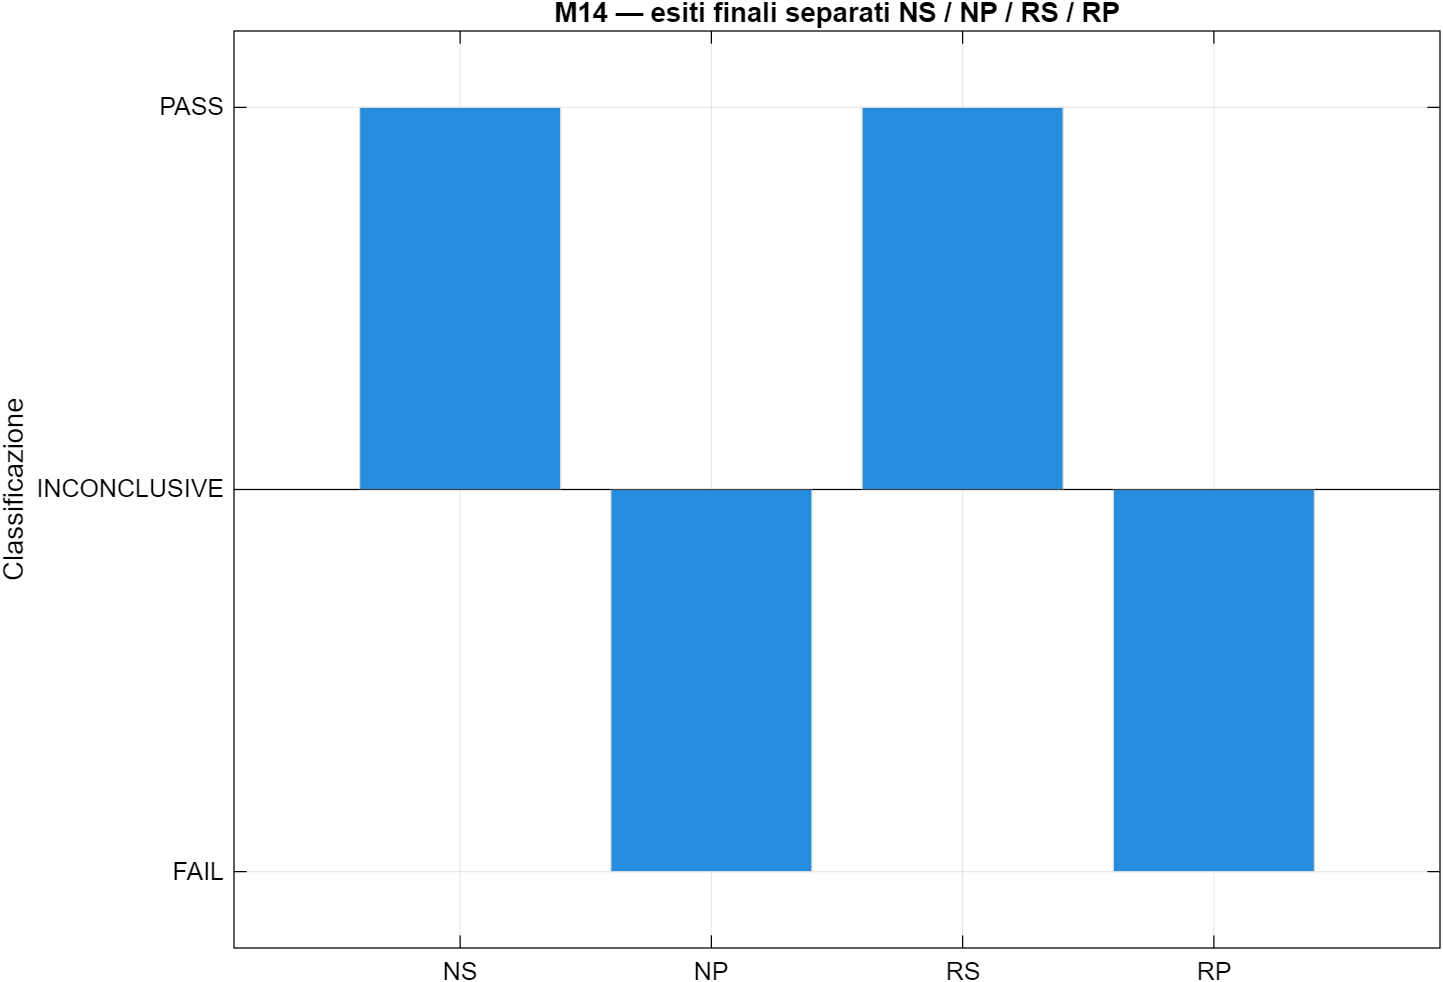
\includegraphics[width=0.38\textwidth]{figures/m14_ns_np_rs_rp_summary.png}
\caption{Esiti distinti di NS, NP, RS e RP per $K_\mu$ nella post-analisi M14.}
\label{fig:m14-summary}
\end{figure}

Il certificato precedente non è trasferibile al nuovo $K_\mu$, né al
modello non lineare. In \texttt{wcgain} la perturbazione restituita è
stabile e realizza il limite inferiore finito: il limite superiore
infinito non dimostra l'instabilità di quella specifica sostituzione.
Restano validi gli esiti negativi indipendenti di RS e RP sopra riportati.
